\documentclass{subfiles}
\begin{document}
%% GENERAL STUDY OF MORSE DOUBLE WELL
\section{General study of the system}
In this secton we will outline the methods used to study our system in general. These studies will be used to set up our system in such a way that our desired configurations are achieved, whilst also ensuring that the system is stable, well-defined and physically meaningful. To this end there are a few things we need to consider:
\begin{itemize}
    \item At what well separation is our approximation of the two particles being distinguishable valid (to a certain degree)?
    \item What parameters do we need to set in order to achieve our desired configurations I and II?
    \item Will our choice of basis functions be sufficient to descibe our system?
    \item How do we ensure that our system is stable, and well-defined - and also physically meaningful?
\end{itemize}
%% Distinguishability of the particles
\subsection{Distinguishability of the particles}\label{sec:distinguishability}
One of the core features of our system - and the foundation of our qubit design - is that the two particles confined in our potential trap act as \emph{distinguishable} particles. As we are looking to trap electrons, indistinguishable particles, we are dealing with fermions, and the Pauli exclusion principle states clearly that two fermions cannot occupy the same quantum state. This fundamental principle would normally prevent us from constructing product states, as the quantum state of any fermionic system must be anti-symmetric under particle exchange.\textcolor{red}{is this really true? and if not, WHEN is it true?}
\\ However, we are assuming that the potential trap can be constructed in such a way that there are minimal correlations between the two particles, and that the wavefunction can be approximated as a product state. In this analysis we shall look at how "distinguishable" (or separable) our system actually is, and find a distance between wells where we can safely assume the particles to be distinguishable. \\ \\
To make an assessment of the systems distinguishability we will firstly look at the eigen-energies of the system given that we either:
\begin{itemize}
    \item Assume the particles to be distinguishable: \\ We construct the wavefunction as a product state
    \begin{align*}
        \Psi(\mathbf{r}_1, \mathbf{r}_2) = \phi_L(\mathbf{r}_1)\otimes\phi_R(\mathbf{r}_2),
    \end{align*} 
    where $\phi_L$ and $\phi_R$ are the single-particle functions located in the left and right well respectivley. We then calculate the energy by diagonalizing the Hamiltonian matrix for this product state system. In such a product state system the Hamiltonian matrix becomes
    \begin{align*}
        H = H_L \otimes I + I \otimes H_R + V,
    \end{align*}
    where $H_L$ and $H_R$ are the single-particle Hamiltonians for the left and right well, and $V$ is the interaction term between the two particles.
    \item Assume the particles to be indistinguishable, and construct a Slater determinant that we solve using Hartree-Fock theory.
\end{itemize}


If we are successful, we should find that for a certain distance between the wells, the "true" distinguishable energy will overlap with the indistinguishable HF-energy. Should this be the case, we can safely assume that the particles behave as distinguishable particles for our intents and purposes. 


%% Optimization of the potential parameters
\subsection{Parameter optimization}\label{sec:optimization_procedure}
As our goal is to realize single-qubit gates and the two-qubit iSwap gate, we need to find suitable configurations of our potential where we achieve the desired degeneracy in energy levels and also our desired level of entanglement between the two particles. As we've discussed in earlier sections the two configurations we are looking for are:
\begin{itemize}
    \item \textbf{Config I}: The measurement configuration, where all energy levels are distinct and there are minimal correlations between the two subsystems (particles). This corresponds to keeping all Von Neumann entropies in our system as close to zero as possible. With this, we know that our two-body energy eigenstates will have a product state structure, and maximal overlap with the Hartree product states $\ket{00}, \ket{01}, \ket{10}, \ket{11}$.
    \item \textbf{Config II}: The entangled configuration, where we have a degeneracy in the energy levels of our system. This degeneracy will give rise to an avoided crossings in the energy spectrum for the first and second energy eigenstates. In this configuration, the 1st and 2nd energy eigenstates are maximally entangled, while the other energy eigenstates are kept as pure as possible (product states). This corresponds to an entropy equal to 1 for $\ket{\phi_1}$ and $\ket{\phi_2}$, and 0 for $\ket{\phi_0}$ and $\ket{\phi_4}$. 
\end{itemize}
As an initial search, we make a grid search over the potential parameters, mostly to map out the landscape of the potential and find regions where we expect to find the desired configuations. Our grid search will be over the following parameters:
\begin{table}
    \centering
    \begin{tabular}{|c|c|c|}
        \hline
        Parameter & Range & Description \\
        \hline
        $D_l, D_r$ & [$D_{\text{min}}$, $D_{\text{max}}$] & The depth of the potential well \\
        $k_l, k_r$ & [$k_{\text{min}}$, $k_{\text{max}}$] & The width of the potential well \\
        $d$ & [$d_{\text{min}}$, $d_{\text{max}}$] & The distance between the two potential wells \\
        \hline
    \end{tabular}
    \caption{The parameters we will search over in our grid search}
\end{table}
with the constraint that $2D / \sqrt{k} < l$ where $l$ are the number of basis functions allocated to each well, as we've discussed earlier. This is to ensure that the basis functions are well within the potential well, and that we do not have any basis functions that are cut off by the potential. This then becomes a \emph{constrained optimization problem}. To perform our optimization we will use the \texttt{scipy.optimize} package, and the \texttt{minimize} function. We will use the \texttt{COBYQA} method, which is a derivative-free optimization method that is well suited for constrained optimization problems. This method is built on the concept of \emph{sequential quadratic programming}, that solves constrained, non-linear problems. For more details on the method, see \cite{razh_cobyqa}. The optimization will be done as follows:
\begin{algorithm}[ht]
\caption{Paramter optimization procedure: High-level overview}
\textbf{Input:}{Parameter ranges \(\mathcal{R}\), \(\epsilon_{\text{coarse}}\), \(\epsilon_{\text{fine}}\)}
\,\,\,\,\textbf{Output:}{Final refined parameter sets}

\textbf{1. Initialization}\\
Generate a collection of random parameter configurations within \(\mathcal{R}\).

\textbf{2. Coarse Optimization}\\
For each configuration in the collection:
\begin{itemize}
  \item Run the optimizer with convergence tolerance \(\epsilon_{\text{coarse}}\).
  \item If the optimized result meets the desired criteria, retain it as a candidate.
\end{itemize}

\textbf{3. Fine Optimization}\\
For each candidate parameter set:
\begin{itemize}
  \item Re‐run the optimizer with tighter tolerance \(\epsilon_{\text{fine}}\).
  \item Add the refined output to the final results.
\end{itemize}

\textbf{4. Return} the final set of optimized parameters.
\end{algorithm}

\subsubsection{Objective function}
An objective function is constructed for the optimizer, which is the object to be minimized by our optimization algorithm. We will have two separate objective functions, one for each configuration we are looking for. Across both configurations, we want to minimize the $\zeta$-parameter, which directly controls the stability of time-evolution through the Hamiltonian matrix. The parameters is defined as 
\begin{equation*}
    \zeta = E_4 - E_1 - E_2 + E_0,
\end{equation*}
and we can identify this as the \emph{accumulated phase} of the rotated time-evolution operator $U = e^{-iHt}$, expressed in terms of the energy eigenstates, $U = \sum_i^4 e^{-iE_it}\ket{\phi_i}\bra{\phi_i}$. We see that written in matrix form in the logical state basis $\{|ij>\}$, this propagator is (where $\ket{11}$ is the 4th energy eigenstate)
\begin{align*}
    U = \begin{pmatrix}
        e^{-iE_{00}t} & 0 & 0 & 0 \\
        0 & e^{-iE_{01}t} & 0 & 0 \\
        0 & 0 & e^{-iE_{10}t} & 0 \\
        0 & 0 & 0 & e^{-iE_{11}t}
    \end{pmatrix}.
\end{align*}
The energy eigenstates themselves are not unique, because we are free to apply arbitrary single-qubit phase rotations to shift their individual phases without affecting populations (as they are cancelled in any innerproduct). By performing local Z-rotations on qubit A and B, we can absorb the phases on the first three states ($\ket{00}$, $\ket{10}$, $\ket{01}$) into $\ket{11}$. In other words, invoking a single global phase, we use single-qubit rotations on each qubit to collect the relative phases onto $\ket{11}$. After the rotations, the condition
\begin{align*}
    E_{11} = E_{10} + E_{01} - E_00
\end{align*}
means that the excitation energy from the 0th state $\ket{00}\to\ket{11}$ equals the sum of excitations $\ket{00}\to\ket{10}$ and $\ket{00}\to\ket{01}$, which aids in ensuring phase stability in our iSwap-like two-qubit gate operation \cite{ku2020suppression}. 
\\\\
Configuration I, as we've mentioned, should have all energy levels distinct. This introduces penalties in our objective function corresponding to the overlap between energy eigenvalues and we want to Von Neumann entropies to be as close to zero as possible. In python we realise this in the following way
\begin{lstlisting}[language=Python]
target_entropy = np.zeros(4)
detuning_penalty = -min(0.5, np.abs(e_L - e_R))
entropy_penalty = np.linalg.norm(entropy - target_entropy)
ZZ_penalty = np.abs(E_4 - E_1 - E_2 + E_0)
\end{lstlisting}
where \texttt{e\_L} and \texttt{e\_R} are the energy levels of the left and right well, and \texttt{entropy} is the Von Neumann entropy of the subsystems. The \texttt{detuning\_penalty} is a penalty that is introduced to ensure that the energy levels are distinct, and the \texttt{entropy\_penalty} is a penalty that ensures that the entropy is as close to zero as possible. The objective function is then the sum of these two penalties. Furthermore, we would like the two configurations parameters to be close in parameter space, so that our evolution between the two configurations is smoooth. We introduce a penalty for this as well, similar to the \texttt{entropy\_penalty}. We also want to penalize off-diagonal coupling terms in the Hamiltonian matrix, as these will introduce unwanted couplings between the subsystems in our measurement configuration. This is done by introducing a \texttt{off\_diagonal\_penalty} that is the scaled sum of the absolute values of the off-diagonal elements in the Hamiltonian matrix.

In configuration II we have a similar detuning penalty, but in this configuration we do want degeneracy in the 1st Hartree energy level in each well, as well as having an entropy penalty, but with a different target vector. We also here want to penalize certain off-diagonal coupling terms in the Hamiltonian matrix that induces unwanted transitions during evolution, and reward the correct coupling between the subsystems that induce entanglement between the first two excited energy eigenstates. This coupling is closely related to the energy difference between said energy states, so we want to minimize $\Delta E_{12} / J_{12}$, where $J_{12}$ is the coupling strength between the first two energy eigenstates through the \texttt{J\_deltaE\_penalty}. 
The objective function is then again the sum of these penalties.
\begin{lstlisting}[language=Python]
target_entropy = np.array([0, 1, 1, 0])
detuning_penalty = np.abs(e_L - e_R)
entropy_penalty = np.linalg.norm(entropy - target_entropy)
ZZ_penalty = np.abs(E_4 - E_1 - E_2 + E_0)
J_12 = np.abs(H[1, 2])  
deltaE_12 = np.abs(E_2 - E_1)  
J_deltaE_penalty = - np.abs(J_12 / deltaE_12 + 1e-12)  
\end{lstlisting}

%%% DVR basis
\subsection{Sinc-Discrete Variable Representation}\label{sec:sinc_dvr_validation}
In this section, we show how to implement the Sinc Discrete Variable Representation (Sinc-DVR) basis used throughout this thesis, and the framework used to validate, and motivate, its usage by comparing the results of the DVR basis against more traditional basis sets, such as the (exact) energy eigenbasis. We do so in a simplified system, where we have a single particle in a Morse potential. This will allow us to compare the results to known analytical solutions. 

As a grid-based basis, Sinc-DVR offers practical computational advantages, particularly when dealing with operators that are diagonally representable and/or localized states. Its effectiveness depends however, on the ability to accurately represent the relevant physical states of the system at hand. To test this, we examine how the DVR basis functions overlap with the exact energy eigenstates of the system, and we use the DVR basis to compute the ground state energy of the system, which we then compare to the result obtained from the exact energy eigenstates by diagonalizaton of the Hamiltonian. 

To validate the Sinc-DVR basis, we compare its performance to the exact energy eigenstates of the system, obtained by directly diagonalizing the Hamiltonian of the system. This mirrors the procedure used to solve the time-independent Schrödinger equation \eqref{eq:tise}, where the eigenvalues and eigenfunctions define the stationary states of the system.

As a test case, we consider a single particle trapped in a Morse potential\eqref{eq:morse_potential}, which models an anharmonic bounded oscillator potential with well-known analytical and numerical solutions. A brief reminder, the Morse potential is given by
\begin{align*}
    V(x) = D \left(1 - e^{-a(x - x_0)}\right)^2,
\end{align*}
where $D$ is the depth of the potential well, $a$ is the width of the potential, and $x_0$ is the equilibrium position of the potential. This potential is well-suited for benchmarking, as it is smooth and localised, and also well represents the more complex double-well potential we are later interested in. It will allow us to compare the DVR-computed energy states to the exact energy eigenstates of the system, and also to test the accuracy of the DVR basis functions in representing the energy eigenstates. Moving on, we will examine both the energy spectrums and the overlap between DVR basis and exact energy eigenstates. 

To summarize, in practice we construct the Sinc-DVR basis by sampling the analytical basis functions $\phi_n(x)$ \eqref{eq:sinc_dvr} over a uniform grid, using standard \texttt{python} libraries such as \texttt{numpy} and \texttt{scipy} for sinc-function evaluation. The grid parameters are chosen to ensure convergence and that the basis functions are well-localized within the potential well, as we will discuss more in following sections. 
\subsubsection*{Energy spectrum} 
The procedure to compute, and compare, the energy spectrum of the Morse potential using the Sinc-DVR basis and the exact energy eigenstates is as follows:
\begin{itemize}
    \item Set up the potential using a set of parameters $D$, $a$, and $x_0$.
    \item Construct the Sinc-DVR basis functions $\phi_n(x)$ over a uniform grid of points $x_i$.
    \item Construct the Hamiltonian matrix $H$.
    \item Diagonalize the Hamiltonian matrix to obtain the energy eigenvalues and eigenstates.
\end{itemize}
We construct the Hamiltonian matrix for the system, using the following expression:
\begin{align*}
    H = -\frac{1}{2} \frac{d^2}{dx^2} + V(x),
\end{align*}
where $V(x)$ is the Morse potential. For the exact energy eigenstates, we can compute the Hamiltonian matrix by discretizing the second derivative operator using finite differences, more specifically, we use the central difference approximation for the second derivative \cite{langtangen2017finite}\footnote{This is a common numerical method for approximating derivatives, and is widely used in numerical analysis. For more details, we refer specifically to ch. 1.1.2 of \cite{langtangen2017finite}.}:
\begin{align}
    \frac{d^2}{dx^2} \approx \frac{f(x + \Delta x) - 2f(x) + f(x - \Delta x)}{\Delta x^2}\label{eq:finite_difference_2nd_derivative}, 
\end{align}
where $\Delta x$ is the grid spacing. As is evident, the approximation \eqref{eq:finite_difference_2nd_derivative} converges to the exact second derivative as $\Delta x \to 0$. The Sinc-DVR kinetic elements are given analytically as in \eqref{eq:sinc_dvr_kinetic}. With these definitions, we have the full one-body Hamiltonian matrix elements for our single particl trapped in a Morse potential.
\\ 
In the following code snippet, we highlight some of the key steps in the construction of the quantum mechanical system and the diagonalization of the Hamiltonian matrix, which is used to obtain the energy eigenstates and eigenvalues of the system. 
\begin{lstlisting}[language=Python, label=lst:dvr_validation]
N = 200
x = np.linspace(-1, 2, N)
dx = x[1] - x[0]

def morse_potential(x, D, a, x0):
    """
    Morse potential function.
    """
    return D * (1 - np.exp(-a * (x - x0)))**2 - D

V_matrix = np.diag(morse_potential(x, D, a, x0))
T_dvr = np.zeros((N, N))
for i in range(N):
    for j in range(N):
        if i == j:
            T_dvr[i, j] = np.pi**2 / (6 * dx**2)
        else:
            T_dvr[i, j] = ((-1)**(i - j)) / (dx**2 * (i - j)**2)
T_exact = np.zeros((N, N))
T_diag = 1 / dx**2 
T_off_diag = -1 / (2 * dx**2)
for i in range(N):
    for j in range(N):
        if i == j:
            T_exact[i, j] = T_diag
        elif abs(i - j) == 1:
            T_exact[i, j] = T_off_diag
        else:
            T_exact[i, j] = 0


H_exact = T_exact + V_matrix
H_dvr = T_dvr + V_matrix
# Diagonalize the Hamiltonian
E_dvr, psi_dvr = np.linalg.eigh(H_dvr)
E_exact, psi_exact = np.linalg.eigh(H_exact)
\end{lstlisting}

\subsubsection*{Energy eigenstates}
To compare the energy eigenstates of the two basis sets, we compute the overlap between the Sinc-DVR basis functions and the exact energy eigenstates of the system. The overlap is defined as
\begin{align*}
    S_{nm} = \braket{\phi_n|\psi_m} = \int_{-\infty}^{\infty} \phi_n(x) \psi_m(x) dx,
\end{align*}
where $\phi_n(x)$ is the Sinc-DVR basis function and $\psi_m(x)$ is the exact energy eigenstate of the system. The overlap can be computed numerically using a direct Riemann sum,
\begin{align*}
    \int_a^b f(x) dx \approx \sum_{i=0}^{N-1} f(x_i) \Delta x, 
\end{align*} 
as shown in the following code snippet, building on the previous code snippet \ref{lst:dvr_validation}:
\begin{lstlisting}[language=Python]
E_dvr, psi_dvr = np.linalg.eigh(H_dvr)
E_exact, psi_exact = np.linalg.eigh(H_exact)
S = np.zeros((n_levels, n_levels))
for i in range(n_levels):
    for j in range(n_levels):
        # Calculate the overlap integral
        overlap = np.sum(psi_dvr[:, i].conj() * psi_exact[:, j])
        S[i, j] = np.abs(overlap)
\end{lstlisting}
where \texttt{n\_levels} is the number of energy levels we are interested in. The reader might notice the lack of $\Delta x$ in the overlap integral, this is due to how \texttt{numpy} produces normalized basis sets from diagonalization in the \texttt{eigh} function, so their (discrete) normalization is already accounted for. The overlap matrix $S$ is then a $n_{\text{levels}} \times n_{\text{levels}}$ matrix, where each element $S_{nm}$ represents the overlap between the $n$th Sinc-DVR basis function and the $m$th exact energy eigenstate of the system. 

The overlap matrix $S$ is then a measure of how well the Sinc-DVR basis functions represent the exact energy eigenstates of the system. The results are shown in figure \ref{fig:dvr_validation_overlap}, where we see that the overlap between the Sinc-DVR basis functions and the exact energy eigenstates is quite high, especially for the lowest lying states. We see that the overlap matrix is close to the identity matrix, indicating a near perfect overlap between the two basis sets.
\begin{figure}[h!]
    \centering
    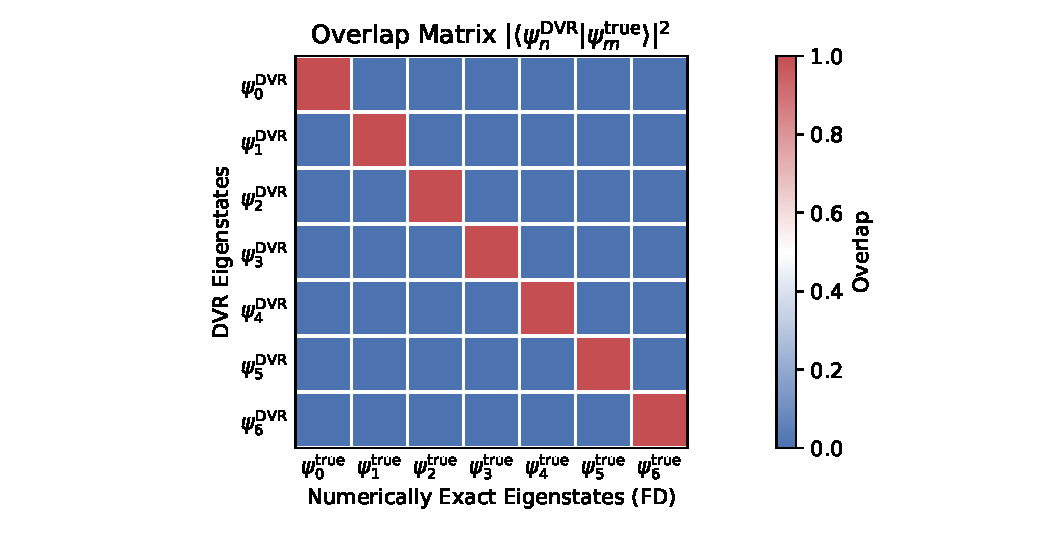
\includegraphics[width=\textwidth]{figs/dvr_validation_overlap.pdf}
    \caption{Overlap between the Sinc-DVR basis functions and the exact energy eigenstates of the Morse potential. The parameters used for the Morse potential are $D = 10.0$, $a = 1.0$, and $x_0 = 0.0$. The grid spacing is $\Delta x = 0.025$, and the number of grid points is $N = 200$.}
    \label{fig:dvr_validation_overlap}
\end{figure}
\\

In summary, we have shown that the Sinc-DVR basis is a valid choice for representing quantum mechanical systems, and that it can be used to accurately compute the energy spectrum and energy eigenstates of the system. We have also shown that the Sinc-DVR basis functions closely match the exact energy eigenstates of the system, especially for the lowest lying states. This gives us confidence in our choice of basis set, and we can safely proceed with our analysis of the double-well potential.

\end{document}